\documentclass[11pt,a4paper]{article}

\usepackage[utf8]{inputenc}
\usepackage[T1]{fontenc}
\usepackage{lmodern}
\usepackage{amsmath,amssymb}
\usepackage{graphicx}
\usepackage{xcolor}
\usepackage{booktabs}
\usepackage[margin=2.5cm]{geometry}
\usepackage[numbers,sort&compress]{natbib}
\usepackage{url}
\usepackage[colorlinks=true,linkcolor=blue!60!black,citecolor=blue!60!black,urlcolor=blue!60!black]{hyperref}
\usepackage{xspace}

\newcommand{\pt}{\ensuremath{p_\mathrm{T}}\xspace}
\newcommand{\HT}{\ensuremath{H_\mathrm{T}}\xspace}
\newcommand{\mjj}{\ensuremath{m_{jj}}\xspace}
\newcommand{\tauTO}{\ensuremath{\tau_{21}}\xspace}
\newcommand{\ptmean}{\ensuremath{\langle \pt \rangle}\xspace}

\begin{document}

\begin{titlepage}
\begin{flushright}
\small Preprint, October 2026
\end{flushright}
\vspace*{1.5cm}
\begin{center}
{\LARGE\bfseries When Graph Autoencoders Look the Wrong Way:\\[0.4em]
\Large Complexity Bias and Simple Baselines in Unsupervised Anomaly Detection on the LHC Olympics 2020 Dataset\par}
\vspace{1.2cm}
{\large Jamil Khan\footnote{\href{mailto:khanjamilahmed202@gmail.com}{khanjamilahmed202@gmail.com}}\par}
\vspace{0.3cm}
{\itshape Independent researcher; undergraduate student in Computer Engineering\par}
\vspace{1.5cm}
\begin{abstract}
\noindent
Graph autoencoders (GAEs) trained only on background are a natural candidate for model-agnostic
new-physics searches. I tested two of them on the LHC Olympics 2020 R\&D dataset, where a
$W'\to XY\to(q\bar q)(q\bar q)$ dijet resonance is hidden in QCD background. The first is a node-level
GAE that scores per-particle reconstruction error. The second encodes the whole event, reconstructs it
with a set decoder and a Chamfer loss, and offers three scores: reconstruction error, latent
$k$-nearest-neighbour distance and latent Gaussian-mixture likelihood. The decision criterion was fixed
before looking at any test result. Neither model beats simple label-free observables. The node-level model reaches an AUC of
$0.483\pm0.005$ with max-reduction and $0.781$ with mean-reduction; all three event-level scores are
\emph{inverted}, with AUCs between $0.401$ and $0.436$, stable across seeds, nine ablations, and
signal-contaminated training. By contrast, the mean transverse momentum per particle,
$\ptmean=\HT/N$, reaches $0.811$, and $-\tauTO$ of the leading jet reaches $0.801$.
Correlation and binned analyses indicate that the latent-density scores track event complexity: the
signal has fewer, harder particles than QCD and is therefore placed in dense regions of the learned
manifold. The benchmark code is public, and I suggest \ptmean as a standard reference baseline for
unsupervised methods on this dataset.
\end{abstract}
\end{center}
\vfill
\noindent\textbf{Code and data:} \url{https://github.com/Viverun/Hidden-Vertex}\\
\textbf{Archived version:} \href{https://doi.org/10.5281/zenodo.23432780}{doi:10.5281/zenodo.23432780}
\end{titlepage}

\section{Introduction}
\label{sec:intro}

Searches for physics beyond the Standard Model (BSM) at the Large Hadron Collider (LHC) are
mostly designed around specific signal hypotheses. Model-agnostic anomaly detection aims to
complement them by flagging events that are atypical with respect to the Standard Model
background, without assuming a signal model. The LHC Olympics 2020 (LHCO)~\cite{Kasieczka:2021xcg}
established a common benchmark for this task, and autoencoders, in which events with large
reconstruction error are treated as anomalous, are among the most widely studied unsupervised
approaches~\cite{Farina:2018fyg,Heimel:2018mkt,Finke:2021sdf,Atkinson:2021nlt}.

Autoencoder scores have a known weakness: they can end up measuring how complex an input is
rather than how unusual it is. For jet images, simple signal jets turn out to be \emph{easier} to
reconstruct than QCD jets~\cite{Finke:2021sdf}. This project started as an attempt to build a
working graph-based detector, and ran into the same problem for particle graphs of whole events.
This paper documents what happened:
\begin{enumerate}
  \item a reproducible benchmark harness on the public LHCO R\&D data, with a frozen test set,
        multi-seed runs, bootstrap confidence intervals and within-bin AUCs that test whether
        a score carries information beyond trivial event quantities;
  \item a set of label-free reference baselines, among which the mean transverse momentum per
        particle, $\ptmean=\HT/N$, is the strongest particle-level observable
        (AUC $0.811$), above \HT, \mjj, and a node-level GAE;
  \item a negative result, under a decision rule fixed in advance, for an event-level GAE whose three anomaly scores are
        systematically inverted, with ablations, a contamination study, and a correlation-based
        diagnosis that links the latent-density inversion to event complexity.
\end{enumerate}
None of this is a working anomaly detector. The practical point is simpler: before claiming that
an unsupervised model has learned something on this dataset, compare it with \ptmean. If it cannot
beat a ratio of two event totals, it has probably only learned the energy and multiplicity scale.

\section{Dataset and test protocol}
\label{sec:data}

I use the LHCO 2020 R\&D dataset~\cite{Kasieczka:2021xcg,LHCO:zenodo}. Background consists of
QCD dijet events and signal of $W'\to XY$ with $m_{W'}=3.5$~TeV, $m_X=500$~GeV and
$m_Y=100$~GeV, each of $X$ and $Y$ decaying to two quarks. Events were generated with
\textsc{Pythia}~8~\cite{Sjostrand:2014zea} and the \textsc{Delphes}~3~\cite{deFavereau:2013fsa}
detector simulation, and are stored as up to 700 hadrons
$(\pt,\eta,\phi)$. Jet-level features (anti-$k_t$~\cite{Cacciari:2008gp} $R=1$ jet masses,
$N$-subjettiness ratios~\cite{Thaler:2010tr} and \mjj) are taken from the accompanying
feature file.

One practical warning first: the publicly available file \texttt{events\_anomalydetection\_v2.h5} is \emph{sorted}: rows
$0$--$999{,}999$ are background and rows $\geq 1{,}000{,}000$ are signal. Any pipeline that
reads a prefix of the file therefore sees no signal at all; I select events explicitly by row
index. The test set is frozen across all experiments: $5{,}000$ background events
(rows $40{,}000$--$44{,}999$) and $5{,}000$ signal events (rows $1{,}000{,}000$--$1{,}004{,}999$).
Models are trained on $180{,}000$ background-only events (rows $\geq 45{,}000$) with a
$20{,}000$-event background validation set.

\paragraph{Metrics.}
I report the ROC AUC with bootstrap confidence intervals over the $10{,}000$ test events
(95\% for baselines; 98.3\% for the three model scores, a Bonferroni correction for three
comparisons). To test whether a score carries information beyond trivial event quantities,
I also compute the AUC \emph{within bins} of \HT, particle multiplicity $N$, and leading-particle
\pt. The sign of every score (``larger = more anomalous'') is fixed in advance.

\paragraph{Decision criterion.}
Before any test result for the event-level model, I fixed the following gate: a model score
passes only if the lower bound of its seed-averaged AUC interval exceeds the best particle-level
baseline, and its minimum within-bin AUC is at least $0.6$.

\section{Models}
\label{sec:models}

\paragraph{Node-level GAE.}
Each event is a radius graph with edges between particles at $\Delta R<0.4$. A graph
convolutional encoder~\cite{Kipf:2016gcn} compresses each particle's features to a one-dimensional
latent and a decoder reconstructs its standardized $(\pt,\eta,\phi)$; the model has 420 effective
parameters. The event score is the maximum or the mean of the per-particle reconstruction
errors.

\paragraph{Event-level GAE.}
The encoder applies three residual neighbour-averaging layers of width 64 on the same
$\Delta R<0.4$ graph, followed by concatenated mean, max and \pt-weighted pooling into a
16-dimensional event latent. A set decoder reconstructs the $K=48$ hardest particles and is
trained with a symmetric Chamfer distance~\cite{Fan:2017chamfer}, which is invariant to particle
ordering. Events are truncated to the 350 hardest particles, a cut chosen from the measured
multiplicity distribution before training ($0.7\%$ of background and $0.02\%$ of signal events
exceed it). The model has $95{,}888$ parameters and is trained for 30 epochs with AdamW
(learning rate $10^{-3}$, batch size 256, early-stopping patience 5) on one NVIDIA T4 GPU,
about 18 minutes per seed. Three anomaly scores are evaluated: (i) the Chamfer reconstruction
error; (ii) the mean distance to the 20 nearest training latents; and (iii) the negative
log-likelihood of the latent under an 8-component Gaussian mixture fitted to training latents.

\section{Results}
\label{sec:results}

\subsection{Reference baselines}

Table~\ref{tab:baselines} lists label-free event observables evaluated on the frozen test set.
The harness reproduces my earlier node-level numbers exactly (\HT $0.792$, \mjj $0.788$,
node-level GAE $0.478$/$0.781$, each inside its interval). The strongest particle-level observable
is \ptmean (AUC $0.811$), which exceeds \HT because it combines the higher energy scale of signal
with its lower multiplicity (mean $N=140$ for signal vs.\ $182$ for background). The
mass-window score $-|\mjj-3500\,\mathrm{GeV}|$ (AUC $0.900$) requires knowledge of the signal and
is shown only as an oracle reference.

\begin{table}[t]
\centering
\caption{ROC AUC of label-free event observables and the node-level GAE on the frozen test set
(5k signal, 5k background), with 95\% bootstrap intervals and the minimum AUC within bins of \HT,
$N$ and leading \pt. Node-level GAE rows are from seed 0; over five seeds the max-reduction AUC is $0.483\pm0.005$.}
\label{tab:baselines}
\begin{tabular}{llccc}
\toprule
Score & Type & AUC & 95\% CI & min.\ within-bin \\
\midrule
$-|\mjj-3500\,\mathrm{GeV}|$ & oracle   & 0.900 & 0.894--0.906 & 0.777 \\
\ptmean $=\HT/N$             & particle & \textbf{0.811} & 0.803--0.821 & 0.599 \\
$-\tauTO$ (leading jet)      & jet      & 0.801 & 0.792--0.810 & 0.664 \\
\HT $=\sum\pt$               & particle & 0.792 & 0.783--0.802 & 0.337 \\
\mjj                         & jet      & 0.788 & 0.778--0.799 & 0.322 \\
Node-level GAE (mean)        & model    & 0.781 & 0.772--0.790 & 0.609 \\
$-N$                         & particle & 0.715 & 0.704--0.726 & 0.399 \\
$m_{j2}$ / $m_{j1}$          & jet      & 0.637 / 0.634 & -- & 0.566 / 0.541 \\
leading-particle \pt         & particle & 0.554 & 0.543--0.565 & 0.388 \\
Node-level GAE (max)         & model    & 0.478 & 0.467--0.489 & 0.376 \\
\bottomrule
\end{tabular}
\end{table}

For the node-level GAE, the choice of reduction matters more than the model: the same trained
network gives $0.48$ with max and $0.78$ with mean. Across five seeds, the max-reduction AUC is
$0.483\pm0.005$. Scaling the network by $44\times$ in parameters lowers the training loss by about
$2\%$ and leaves the AUC unchanged. The max score is dominated by the hardest particle
(Spearman $\rho=0.70$ with leading \pt, and AUC $0.38$--$0.47$ within leading-\pt deciles).
Since a per-particle MLP with the same one-dimensional bottleneck reconstructs \pt almost
perfectly, the residual error originates in the neighbourhood averaging of the graph convolution.
The mean score retains AUC $0.61$--$0.82$ within deciles of \HT, $N$ and leading \pt, but it is
strongly anti-correlated with multiplicity ($\rho=-0.71$) and does not exceed \ptmean.

\subsection{Event-level GAE}

Table~\ref{tab:event} summarises the headline result. All three scores lie significantly
\emph{below} $0.5$, and the gate is not passed. The seed-to-seed spread (0.01--0.02) is small
compared with the distance to $0.5$, so the inversion is systematic. Training was stable, with
agreement between training and validation loss and no latent collapse.

\begin{table}[t]
\centering
\caption{Event-level GAE: seed-averaged AUC over three seeds with 98.3\% bootstrap intervals,
minimum within-bin AUC, and per-seed values.}
\label{tab:event}
\begin{tabular}{lcccc}
\toprule
Score & AUC & 98.3\% CI & min.\ within-bin & seeds 0 / 1 / 2 \\
\midrule
Chamfer reconstruction & 0.428 & 0.415--0.442 & 0.311 & 0.419 / 0.433 / 0.432 \\
Latent $k$NN distance  & 0.401 & 0.389--0.412 & 0.281 & 0.405 / 0.397 / 0.401 \\
Latent GMM likelihood  & 0.436 & 0.426--0.448 & 0.308 & 0.448 / 0.427 / 0.434 \\
\bottomrule
\end{tabular}
\end{table}

Figure~\ref{fig:summary} compares all scores. Every model score lies below the simplest
particle-level observables.

\begin{figure}[t]
\centering
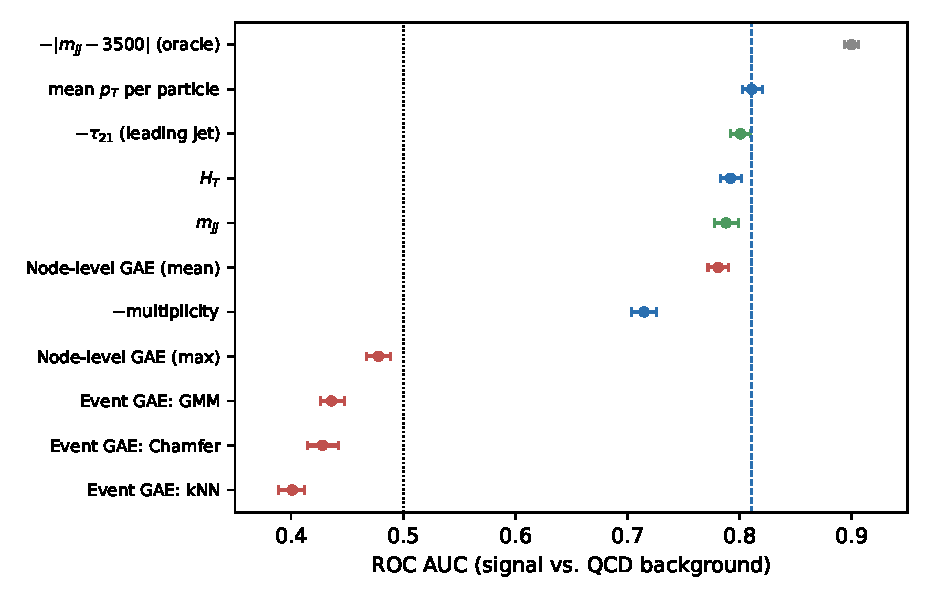
\includegraphics[width=0.78\textwidth]{figures/auc_summary.pdf}
\caption{ROC AUC with confidence intervals for reference observables (blue: particle level;
green: jet level; grey: oracle) and autoencoder scores (red). The dotted line marks chance and
the dashed line the \ptmean baseline.}
\label{fig:summary}
\end{figure}

\subsection{Ablations and contamination}

Nine variations of the event-level model, each with two seeds, were run as a sensitivity
analysis and not used to select a configuration (Table~\ref{tab:ablation}). None produces a
useful score; the best single value is $0.502$ (Chamfer, $K=24$), i.e.\ chance. Training on
background contaminated with $1\%$ signal changes the scores by at most $\sim0.015$, which is
inconclusive with one seed. At $9\%$ contamination, the signal fraction of the R\&D file, the
density scores become \emph{more} inverted ($k$NN $0.362$, GMM $0.387$), consistent with signal
events making signal-like regions of the latent space denser.

\begin{table}[t]
\centering
\caption{Sensitivity of the event-level GAE (seed-averaged AUC). Main configuration: latent 16,
$K=48$, depth 3, full pooling, unweighted Chamfer loss. Contamination rows use one seed.}
\label{tab:ablation}
\begin{tabular}{lcccc}
\toprule
Variant & seeds & Chamfer & $k$NN & GMM \\
\midrule
main                           & 3 & 0.428 & 0.401 & 0.436 \\
latent 4                       & 2 & 0.366 & 0.405 & 0.403 \\
latent 8                       & 2 & 0.401 & 0.372 & 0.376 \\
latent 32                      & 2 & 0.428 & 0.412 & 0.485 \\
$K=24$                         & 2 & 0.502 & 0.447 & 0.475 \\
$K=96$                         & 2 & 0.490 & 0.425 & 0.447 \\
depth 2                        & 2 & 0.421 & 0.412 & 0.442 \\
depth 4                        & 2 & 0.429 & 0.388 & 0.428 \\
no \pt-weighted pooling        & 2 & 0.424 & 0.408 & 0.451 \\
\pt-weighted Chamfer loss      & 2 & 0.475 & 0.454 & 0.468 \\
\midrule
pure background (seed 0)       & 1 & 0.419 & 0.405 & 0.448 \\
1\% signal in training         & 1 & 0.424 & 0.420 & 0.461 \\
9\% signal in training         & 1 & 0.413 & 0.362 & 0.387 \\
\bottomrule
\end{tabular}
\end{table}

\section{Diagnosis}
\label{sec:diagnosis}

Table~\ref{tab:corr} gives Spearman correlations of the seed-0 scores with simple event
quantities. The latent-density scores increase with multiplicity ($\rho=+0.28$ for $k$NN,
$+0.23$ for GMM) and decrease with \ptmean ($-0.27$, $-0.20$), also within background alone. Their
AUC within multiplicity bins is close to chance ($k$NN $0.43$--$0.50$, GMM $0.47$--$0.51$).
Since signal events have fewer and harder particles than QCD background, they fall into dense
regions of a latent space trained on QCD. Under the pre-declared sign (far from training data
means anomalous), this produces AUCs below $0.5$. This explanation is supported by correlations
but was not tested causally.

The Chamfer score behaves differently: it barely tracks multiplicity ($\rho=+0.08$) or \ptmean
($\rho=-0.07$), and remains inverted within multiplicity bins ($0.41$--$0.48$) and within \HT
bins (down to $0.31$). Its inversion is therefore not explained by multiplicity alone, and its
origin remains open. The three scores are only moderately correlated with one another (Chamfer--$k$NN
$0.53$, Chamfer--GMM $0.42$, $k$NN--GMM $0.87$). Flipping the sign post hoc would give AUCs of
$0.56$--$0.60$, still far below \ptmean. I mention this only to show that the scores contain a
weak complexity signal rather than noise; it is not a result.

\begin{table}[t]
\centering
\caption{Spearman correlation of seed-0 event-level scores with event quantities
(all test events / background only / signal only).}
\label{tab:corr}
\footnotesize\setlength{\tabcolsep}{4pt}
\begin{tabular}{lcccc}
\toprule
Score & \HT & $N$ & leading \pt & \ptmean \\
\midrule
Chamfer & $-0.01$ / $+0.15$ / $0.00$ & $+0.08$ / $+0.08$ / $-0.01$ & $+0.17$ / $+0.18$ / $+0.19$ & $-0.07$ / $-0.02$ / $+0.01$ \\
$k$NN   & $-0.02$ / $+0.19$ / $0.00$ & $+0.28$ / $+0.30$ / $+0.19$ & $-0.02$ / $-0.05$ / $+0.05$ & $-0.27$ / $-0.24$ / $-0.20$ \\
GMM     & $+0.02$ / $+0.18$ / $0.00$ & $+0.23$ / $+0.27$ / $+0.15$ & $+0.01$ / $-0.04$ / $+0.09$ & $-0.20$ / $-0.21$ / $-0.16$ \\
\bottomrule
\end{tabular}
\end{table}

\section{Discussion and outlook}
\label{sec:discussion}

These results add to the evidence that autoencoder-based anomaly scores are vulnerable to
complexity bias~\cite{Finke:2021sdf}, and extend it to particle-graph representations of
full events. Two practical lessons follow. First, unsupervised methods on the LHCO R\&D data
should be compared not only with \HT but with \ptmean, which already reaches AUC $0.81$ without
any training. Second, within-bin AUCs at fixed multiplicity and \HT are a cheap and informative
diagnostic: a score that loses its discrimination at fixed complexity has not learned
substructure.

The features that distinguish the signal in this dataset are jet-level: two-prong
substructure (\tauTO), jet masses and \mjj. These are not available to the encoder as explicit
inputs. Natural next steps are therefore (i) adding jet-level and substructure inputs,
(ii) conditioning the model on, or regressing out, multiplicity and \ptmean so that the score
measures structure at fixed complexity, and (iii) choosing the score sign on background-only or
simulated data. Large foundation models for collider physics trained on simulated events are
expected to face the same issue. Benchmarks of the kind released here can be used to check
whether their anomaly scores capture more than event complexity.

\paragraph{Limitations.}
All results use a single signal model and the R\&D dataset, not the LHCO black boxes. The
event-level model was evaluated in one configuration fixed in advance with limited ablations,
and the complexity explanation is correlational. Ablation and contamination runs use two or
one seeds, so differences below $\sim0.02$ should not be interpreted.

\section*{Code availability}
All code, configurations, and the benchmark harness are available at the public repository
\url{https://github.com/Viverun/Hidden-Vertex}, under the MIT licence. The detailed result
reports are in \texttt{docs/PART1\_VERIFICATION.md} and \texttt{docs/PART2\_RESULTS.md}.

\section*{Acknowledgements}
I thank the organisers of the LHC Olympics 2020 for making the dataset public. Computations
were performed on Kaggle GPU notebooks.

\section*{Use of AI tools}
AI assistants (Anthropic's Claude) were used to help with code development, debugging and
editing of the manuscript text. All experiments, results and conclusions were checked by the
author, who takes full responsibility for the content of this paper.

\bibliographystyle{unsrtnat}
\bibliography{refs}

\end{document}
